\documentclass[12pt,fleqn]{article}\usepackage{../../common}
\begin{document}
Materyel Mekaniği - 3

Bükülen bir çubuğun formüllerine bir giriş [1] kaynağında yapıldı. Orada
moment-eğri (moment-curvature) formülü gösterilmişti.

$$
M(x) = \frac{E(x)I(x)}{\rho(x)}
\mlabel{1}
$$

Şimdi bu formülü genişletelim, ve bir ikinci derece türeve eşitleyelim.

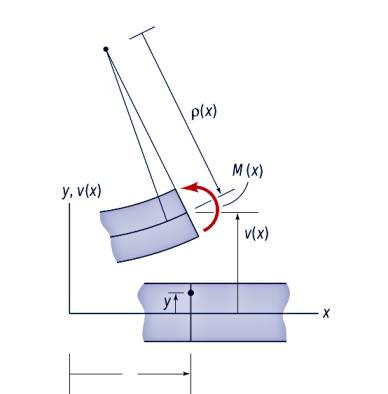
\includegraphics[width=15em]{phy_020_strs_05_01.jpg}

Resimde gösterilen semboller $M$ bükme momenti, $\rho$ çubuğun $+y$ tarafındaki
bükülme çemberinin, eğiminin yarıçapı (radius of curvature).  $v$ ise yine $+y$
kısmındaki yer değişimidir. Çubuğa uygulanan kuvvet dağılımının ne olduğu
önemli değil, sonuçta odaklandığımız çubuğun ufak bir kısmı.

[7] kaynağında bir çemberi (yarıçapını) onun bir eğriye dokunduğu noktadaki
türevler üzerinden temsil etme tekniğini paylaştık. Bu formülü mevcut probleme
uygulayabiliriz.

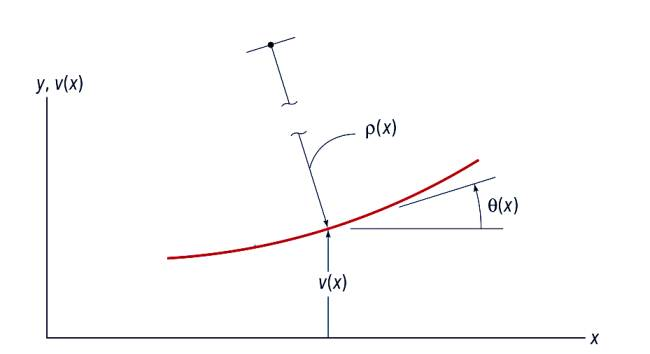
\includegraphics[width=20em]{phy_020_strs_05_02.jpg}

Üstteki örnekte çemberin yarıçapı $\rho$, türevler ise $\ud v / \ud x$.
Formül [6, sf. 466],

$$
\frac{1}{\rho} =
\frac
{\dfrac{\ud^2 v}{\ud x^2}}
{ \left[ 1 + \left( \dfrac{\ud v}{\ud x}  \right)^2 \right]^{3/2} }
$$

Üstteki problemde eğim çok ufaktır o zaman $\ud v / \ud x$ ufak kabul edilir
(resimdeki eğim eğitim amaçlı abartılmış), demek ki bölendeki kare hesabı
daha da ufalır, geriye sadece 1 kalır, 1 ile bölümü yok sayarız, geriye kalanlar

$$
\frac{1}{\rho} \approx \frac{\ud^2 v}{\ud x^2}
\mlabel{2}
$$

Şimdi (1) formülünü tekrar düzenlersek,

$$
\frac{1}{\rho} = \frac{M}{EI }
$$

diyebilirdik. Bu formülün sol tarafının (2) sol tarafı ile aynı olduğunu
görüyoruz. Demek ki onları eşitleyebiliriz, moment-eğri formülü şu hale gelir,

$$
\frac{\ud^2 v}{\ud x^2} = \frac{M}{E I}
$$

Formüller daha kısa olsun diye bazı notasyonel ekler yapalım,

$$
v' = \frac{\ud v}{\ud x} \quad 
v'' = \frac{\ud^2 v}{\ud x^2} \quad 
M' = \frac{\ud M}{\ud x} \quad 
$$

İki üstteki formül kısa notasyonla söyle olur,

$$
EI v'' = M
\mlabel{3}
$$

Bir formül daha, sonra faydalı olacak, hatırlarsak,

$$
v = \frac{\ud M}{\ud x}
$$

idi, o zaman (3)'teki formülün iki tarafının $x$'e göre türevini alırsak,

$$
EI v''' = \frac{\ud M}{\ud x} = V
$$

Yani [5, sf. 683]

$$
v = EI v''' = EI \frac{\ud^3 v}{\ud x^3}
\mlabel{6}
$$

Ayrıca [4]'de gösterilmişti, $\ud v / \ud x = -q$ olduğu için

$$
EI v'''' = \frac{\ud v}{\ud x} = -q
$$

ifadesi de doğrudur.




















Euler-Bernoulli kirişlerini temel alan analizleri üç adıma bölmek mümkündür.

1) Uygulanan yük $q$'yu kullanarak saptırma (deflection) fonksiyonu $y$'yi hesapla,

$$
q = E I \frac{\ud^4 y}{\ud X_1^4}
$$

Formülde görüyoruz eğer $q$ biliniyorsa ve elde yeterli sınır şartları var ise
(dört tane) diferansiyel denklemi kullanarak $y$'yi bulabiliriz
[1, Lecture 2, 2:02:00]. 

2) Saptırma $y$ bulunduktan sonra onu kullanarak kaykılma (shear) ve bükülme
momentini hesapla,

$$
M = E I \frac{\ud^2 y}{\ud X_1^2}, \quad
V = E I \frac{\ud^3 y}{\ud X_1^3} 
$$

çünkü sonuçta $M,V$ hesapları $y$'nin birer fonksiyonu, elde edilen $M,V$
sonuçları $X_1$'in fonksiyonları olacak tabii ki.

3) Oradan hareketle moment ve kaykılma $M,V$ bulunanca stres bileşenlerini
bulabilirim,

$$
\sigma_{11} = -\frac{M X_2}{I}, \quad
\sigma_{12} = -\frac{VQ}{I b}
\mlabel{2}
$$

Soru

Alttaki 6 metreli Euler-Bernoulli kirişinin uygulanan $q$ yükü sebebiyle sahip
olacağı yer değişim fonksiyonunu bulun. Kirişin Young genliği 20,000 MPa, ve ona
eşit şekilde dağılmış bir 45 kN / m $q$ yükü uygulanıyor, kalınlığı 600 mm,
yüksekliği 800 mm.

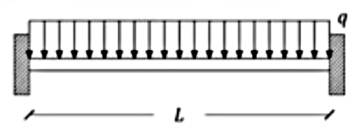
\includegraphics[width=20em]{phy_020_strs_03_02.jpg}

Çözüm

Bir dikdörtgenin atalet momenti $b h^3 / 12$. EI tabii ki Young'in genliği çarpı
bu sayı olur. Aradığımız $y$ denklemi, dördüncü dereceden bir diferansiyel
denklem çözeceğiz. Dördüncü derece demek nihai çözüm için dört tane sınır
şartı gerekli demek. Bu şartları vermeden çözersek,

\begin{minted}[fontsize=\footnotesize]{python}
import sympy as sym
L = 6000 # mm bazinda
Em = 20000
b = 500
h = 800
Ig = (b * h**3)/12
EI = Em * Ig
q = -25 # Newton icin 1000 carpip mm icin 1000 ile bolduk ayni kaldi
X1, X2 = sym.symbols('X1, X2')
y = sym.Function('y')
sol = sym.dsolve(EI*y(X1).diff(X1,4)-q, y(X1))
print (sym.latex(sol))
\end{minted}

\begin{verbatim}
y{\left(X_{1} \right)} = C_{1} + C_{2} X_{1} + C_{3} X_{1}^{2} + C_{4} X_{1}^{3} - \frac{25 X_{1}^{4}}{10240000000000008}
\end{verbatim}

Çağrı \verb!dsolve! sıfıra eşitlik faraziyesi ile hareket ediyor, bu sebeple
üstteki çağrıda diferansiyel denklemin neye eşit olduğunu berlirtmedik, sıfıra
eşitlik farz edildi.

$$
y{\left(X_{1} \right)} = C_{1} + C_{2} X_{1} + C_{3} X_{1}^{2} + C_{4} X_{1}^{3} - \frac{25 X_{1}^{4}}{10240000000000008}
$$

$X_1^4$ katsayısı [1, Lecture 2]'de 1 bölü büyük bir sayı olarak gösterilmiş,
acaba aynı sonuca vardık mı? Kontrol edelim,

\begin{minted}[fontsize=\footnotesize]{python}
print (1/(25./10240000000000008.))
\end{minted}

\begin{verbatim}
409600000000000.3
\end{verbatim}

Katsayı aynı. Gördüldüğü gibi çözümde 4 tane sabit var, bu sabitler orada çünkü
sınır şartlarını tanımlamadık. Onlar tanımlanınca sabitler yokolacak,

\begin{minted}[fontsize=\footnotesize]{python}
y1 = y(X1).subs(X1,0)
y2 = y(X1).subs(X1,L)
th = y(X1).diff(X1)
th1 = th.subs(X1,0)
th2 = th.subs(X1,L)
sol = sym.dsolve(EI*y(X1).diff(X1,4)-q, y(X1),ics={y1:0,y2:0,th1:0,th2:0})
print (sym.latex(sol))
\end{minted}

\begin{verbatim}
y{\left(X_{1} \right)} = - \frac{25 X_{1}^{4}}{10240000000000008} + \frac{12500 X_{1}^{3}}{426666666666667} - \frac{37500000 X_{1}^{2}}{426666666666667}
\end{verbatim}

$$
y{\left(X_{1} \right)} = - \frac{25 X_{1}^{4}}{10240000000000008} + \frac{12500 X_{1}^{3}}{426666666666667} - \frac{37500000 X_{1}^{2}}{426666666666667}
$$

Şimdi kaykılma $V$ ve moment $M$ hesaplanabilir, bu fonksiyonlar $y$'nin farklı
derecedeki türevlerini içeriyor, 

\begin{minted}[fontsize=\footnotesize]{python}
y = sol.rhs
V = EI * y.diff(X1,3)
M = EI * y.diff(X1,2)
print (V)
print (M)
\end{minted}

\begin{verbatim}
74999.9999999999 - 25.0*X1
-12.5*X1**2 + 74999.9999999999*X1 - 74999999.9999999
\end{verbatim}

Stres öğesini hesaplayabilirim şimdi, formülleri (2)'de,

\begin{minted}[fontsize=\footnotesize]{python}
S11 = -M * X2 / Ig
print (sym.simplify(S11))
\end{minted}

\begin{verbatim}
X2*(5.85937499999999e-10*X1**2 - 3.515625e-6*X1 + 0.003515625)
\end{verbatim}

\begin{minted}[fontsize=\footnotesize]{python}
Q = b*((h/2) - X2) * ((h/2)+(X2/2))
S12 = (-V * Q) / (Ig*b)
print (S12)
\end{minted}

\begin{verbatim}
9.375e-14*(200000.0 - 500*X2)*(25.0*X1 - 74999.9999999999)*(X2/2 + 400.0)
\end{verbatim}

Yer değişim sonucunu grafikleyelim,

\begin{minted}[fontsize=\footnotesize]{python}
u = sym.lambdify(X1, y,'numpy')
x = np.linspace(0,L,20)
plt.plot(x,u(x))
plt.title(u'Yer Değişim y')
plt.savefig('phy_020_strs_03_03.jpg',quality=30)
\end{minted}

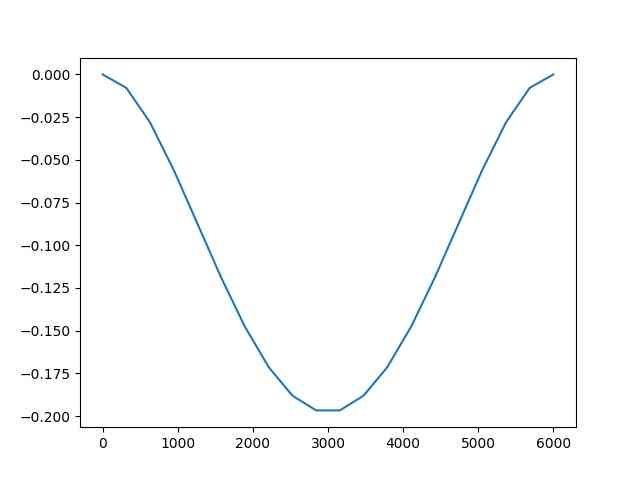
\includegraphics[width=20em]{phy_020_strs_03_03.jpg}

Akla yatkın, ortalara doğru kirişin bükülmesi daha fazla her iki yana doğru daha
az.

Kaykılma ve momenti de grafikleyelim,

\begin{minted}[fontsize=\footnotesize]{python}
v = sym.lambdify(X1, V,'numpy')
x = np.linspace(0,L,20)
plt.plot(x,v(x))
plt.title(u'Kaykılma, V')
plt.savefig('phy_020_strs_03_04.jpg',quality=30)
\end{minted}

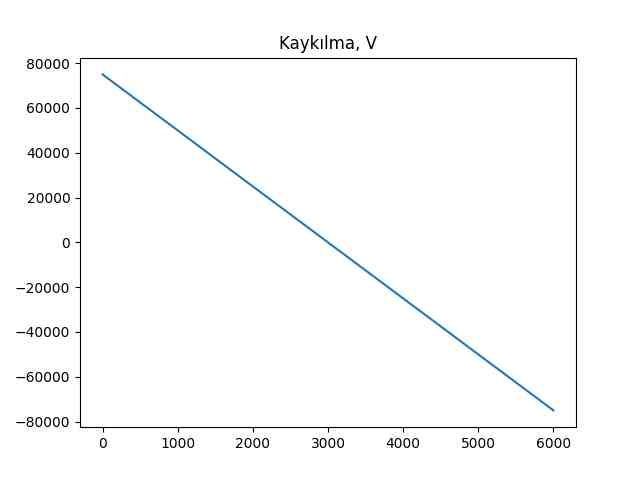
\includegraphics[width=20em]{phy_020_strs_03_04.jpg}

\begin{minted}[fontsize=\footnotesize]{python}
m = sym.lambdify(X1, M,'numpy')
x = np.linspace(0,L,20)
plt.plot(x,m(x))
plt.title('Moment, M')
plt.savefig('phy_020_strs_03_05.jpg',quality=30)
\end{minted}

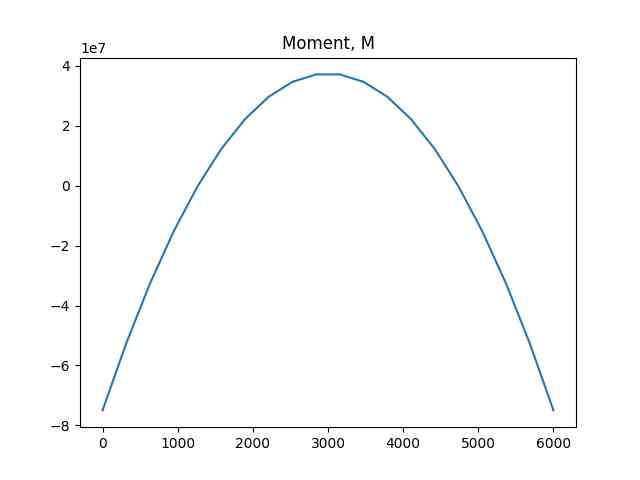
\includegraphics[width=20em]{phy_020_strs_03_05.jpg}

\begin{minted}[fontsize=\footnotesize]{python}
s11f = sym.lambdify([X1,X2], S11,'numpy')
x = np.linspace(0,L,20)
y = np.linspace(-h/2,h/2,20)
xg,yg = np.meshgrid(x,y)
zg = s11f(xg,yg)
plt.contourf(xg,yg,zg,cmap='gnuplot2')
plt.savefig('phy_020_strs_03_06.jpg',quality=30)
\end{minted}

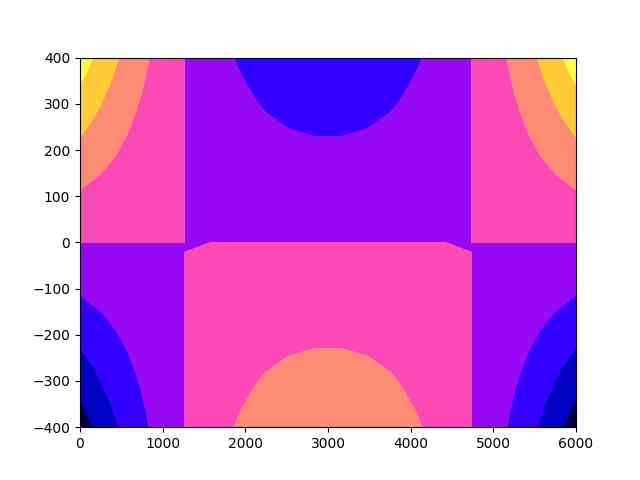
\includegraphics[width=20em]{phy_020_strs_03_06.jpg}

Yine akla yatkın; grafiğin üst kısımda koyu maviye yakın yerde sıkışma
(compression) var orada materyel daralma, içe doğru baskı yaşıyor. Alt kısımda
ise gerginlik var, burada materyel yanlara doğru çekiliyor. Desteklere yakın
noktalarda alt sol ve sağda sıkışma görüyoruz, onun üstünde gerginlik.
Bunlar da mantıklı.

Kaynaklar

[1] Petitt, {\em Intro to the Finite Element Method}, University of Alberta,
    \url{https://www.youtube.com/watch?v=2iUnfPRk6Ro&list=PLLSzlda_AXa3yQEJAb5JcmsVDy9i9K_fi}

[2] Gramoll, {\em Mechanics},
    \url{http://www.ecourses.ou.edu/cgi-bin/ebook.cgi?topic=me}

[3] Bayramlı, {\em Fizik, Materyel Mekaniği - 1}
    
[4] Bayramlı, {\em Fizik, Materyel Mekaniği - 2}

[5] Gere, {\em Mechanics of Materials}

[6] Craig, {\em Mechanics of Materials, Third Edition}

[7] Bayramlı, {\em Çok Değişkenli Calculus, Eğrilik (Curvature)}

\end{document}

